\chapter{MARCO TEÓRICO}\label{chap:marco}
\vskip 3.0ex

En este capítulo se presentan las definiciones de grafos y cliques maximales, y codificaciones ocupadas en este trabajo.

\section{Grafos y cliques maximales} \label{marco:grafoclique}
Se define un \textbf{grafo} $G = (V, E)$ como el conjunto finito de \textit{vértices} o \textit{nodos} $V$ y el conjunto de \textit{aristas} $E \subseteq V \times V$ (arcos). La expresión $V(G)$ representa el conjunto de sus vértices y $E(G)$ el conjunto de sus aristas. El \textit{orden} de un grafo corresponde al total de sus vértices $|V(G)|$, mientras que el \textit{tamaño} de un grafo corresponde al total de sus aristas $|E(G)|$. 

Dos vértices $v_{1}$ y $v_{2} \in V(G)$ son \textbf{adyacentes} o \textbf{vecinos} si $(v_{1}, v_{2}) \in E(G)$ y $v_{1} \neq v_{2}$.  Un grafo es \textbf{no dirigido} cuando la arista conlleva ambos sentidos, quiere decir que $(v_{1}, v_{2}) = (v_{2}, v_{1})$, ambos vértices son vecinos directos entre sí. Caso aparte son los grafos \textbf{dirigidos}, donde las aristas tienen un solo sentido, y $(v_{1}, v_{2}) \neq (v_{2}, v_{1})$. En este caso, $v_{2}$ es llamado \textbf{vecino directo} de $v_{1}$, mientras $v_{1}$ es llamado \textbf{vecino inverso o reverso} de $v_{2}$. Un \textbf{grafo denso} es aquel que su número de aristas es cercano al máximo. Este trabajo está enfocado a utilizar grafos no dirigidos y poco densos. 

El \textbf{grado de un vértice} $d(v)$ se define como la cantidad de vértices en $V(G)$ que son adyacentes con $v$. La \textbf{matriz de adyacencia} de un grafo $G$ corresponde a una matriz binaria cuadrada $|V(G)| \times |V(G)|$ donde cada bit representa si un par de vértices $v_{1}$ y $v_{2} \in V(G)$ son vecinos o no. En resumen, todos sus valores son ceros a menos que haya una arista entre dichos vértices.

Un grafo \textbf{k-degenerate} es no dirigido, donde cada subgrafo tiene un vértice con grado a lo más \textbf{k}. El índice de \textbf{degeneracy} de un grafo, $D(G)$, es el menor valor \textbf{k} para el cual el grafo es \textbf{k-degenerate}.

\begin{figure}
    	\centering
    	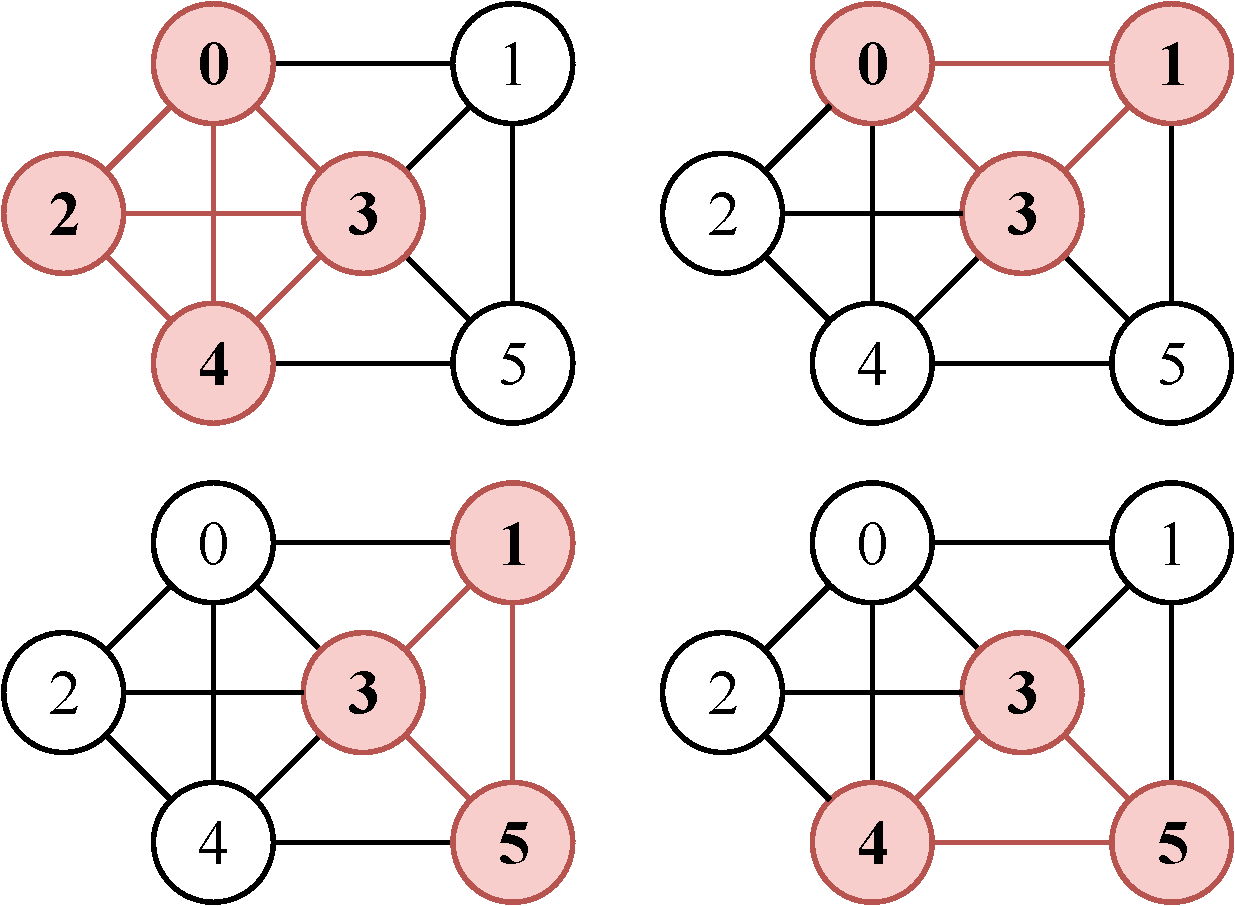
\includegraphics[width=0.5\linewidth]{img/maxCliqueExample.pdf}
    	
    \caption{Ejemplo de grafo y sus cliques maximales.}
    \label{fig:maxCliqueExample}
\end{figure}


Un \textbf{clique} es un subgrafo donde todos los vértices son adyacentes entre sí, es decir, $\exists V' \subseteq V(G), \forall v_{1}, v_{2} \in V', (v_{1}, v_{2}) \in E(G) $. Un \textbf{clique maximal} no puede extenderse incluyendo otro vértice adyacente, es decir, no es subconjunto de otro clique más grande. En la Figura~\ref{fig:maxCliqueExample} se presenta ejemplo de un grafo y sus cliques maximales.

Un \textbf{triángulo} es un subgrafo de tres vértices y tres aristas. Se define $\lambda(v)$ como la cantidad de triángulos donde participa un nodo $v$, y $\lambda(G)$ como la cantidad de triángulos de un grafo, y se calcula sumando el cálculo individual para cada vértice, y dividiendo el total en tres (por cada triángulo se cuentan 3 veces los vértices), como lo muestra la siguiente ecuación

\begin{equation}
	\lambda(G) = \dfrac{1}{3} \sum_{v \in V} \lambda(v) \label{eq:triangles}
\end{equation}

Un \textbf{triplete} es un subgrafo de tres vértices y dos aristas, donde las aristas comparten un vértice común. Se define $\tau(v)$ como la cantidad de tripletes donde $v$ es el vértice común, y $\tau(G)$ como la cantidad de tripletes de un grafo.

\begin{equation}
	\tau(G) = \sum_{v \in V} \tau(v) \label{eq:triplets}
\end{equation}

El \textbf{coeficiente de clusterización} de un vértice indica cuánto está conectado con sus vecinos, y se define como $c(v) =  \lambda(v) / \tau(v)$. El coeficiente de clusterización de un grafo ($C(G)$) es el promedio del coeficiente de todos los nodos del grafo, y se define como:

\begin{align}
	C(G) &= \dfrac{1}{|V'|} \sum_{v \in V'} c(v) \label{eq:CC} \\
	V' &= \{ v \in V | d(v) \geq 2 \} \nonumber
\end{align}

\noindent donde $V'$ es el conjunto de vértices con un grado mayor a dos. Su rango es entre $[0, 1]$, mientras más cercano a $1$ indica más conexión entre vértices.

La \textbf{transitividad} de un grafo ($T(G)$) es la probabilidad que un par de nodos adyacentes estén interconectados, y se define como:

\begin{equation}
	T(G) = \dfrac{3 \lambda(G)}{\tau(G)} \label{eq:T} 
\end{equation}

\noindent y su rango también va entre $[0, 1]$, siendo $1$ cuando todos los nodos están interconectados con todos.

Tanto el coeficiente de clusterización como la transitividad son métricas que permiten vislumbrar cuán conectados o clusterizados están los vértices de un grafo, y de sus ecuaciones se puede notar que están relacionados.

\section{Codificaciones}\label{sec:coding}
Una codificación muy usada es la propuesta por Huffman\cite{huffman1952method}, que retorna códigos de largo variable. Su conversión se basa en la frecuencia de los símbolos en la secuencia de entrada, codificando los más frecuentes con menos bits. Esta representación requiere tanto la secuencia codificada junto a un vocabulario de símbolos para recuperar la secuencia original. 

En la Figura~\ref{fig:huffman} se muestra un ejemplo de esta codificación, donde (a) es la secuencia de entrada, (b) es la secuencia de salida, y (c) es el vocabulario de símbolos dispuesto en un árbol binario. Primero se cuenta la frecuencia de cada símbolo en la secuencia de entrada, dos veces $1$, dos veces $2$, y cinco veces $3$. Luego se crea el árbol binario, partiendo por las hojas de los símbolos menos frecuentes, $1$ y $2$, y creando un nodo con la frecuencia total de ambos casos, en total cuatro. Luego esa rama se añade a otro nodo junto con la hoja del símbolo más probable, $3$, y ambas suman la frecuencia total de nueve símbolos. Así, el símbolo $3$ puede representarse tan solo con un bit en 1, y para los otros casos se necesitarán dos bits.

Para recuperar la secuencia original, se debe recorrer la de salida bit a bit de izquierda a derecha, e ir avanzando en el árbol binario hasta llegar a una hoja. Una desventaja de este método es que necesita decodificar de manera secuencial todo el código para obtener la secuencia original.

\begin{figure}%[b]
    	\centering
    	\begin{minipage}{0.45\textwidth}
    		\centering

		\textbf{\large \textcolor{color3}{3}\textcolor{color2}{2}\textcolor{color3}{3}\textcolor{color3}{3}\textcolor{color1}{1}\textcolor{color2}{2}\textcolor{color3}{3}\textcolor{color1}{1}\textcolor{color3}{3}}
    		
    		(a)
		\vspace{10mm}  		
    		
    		\textbf{\large \textcolor{color3}{1}\textcolor{color2}{01}\textcolor{color3}{1}\textcolor{color3}{1}\textcolor{color1}{00}\textcolor{color2}{01}\textcolor{color3}{1}\textcolor{color1}{00}\textcolor{color3}{1}}
    		
    		(b)
    	\end{minipage}
    	\begin{minipage}{0.45\textwidth}
    		\centering
    		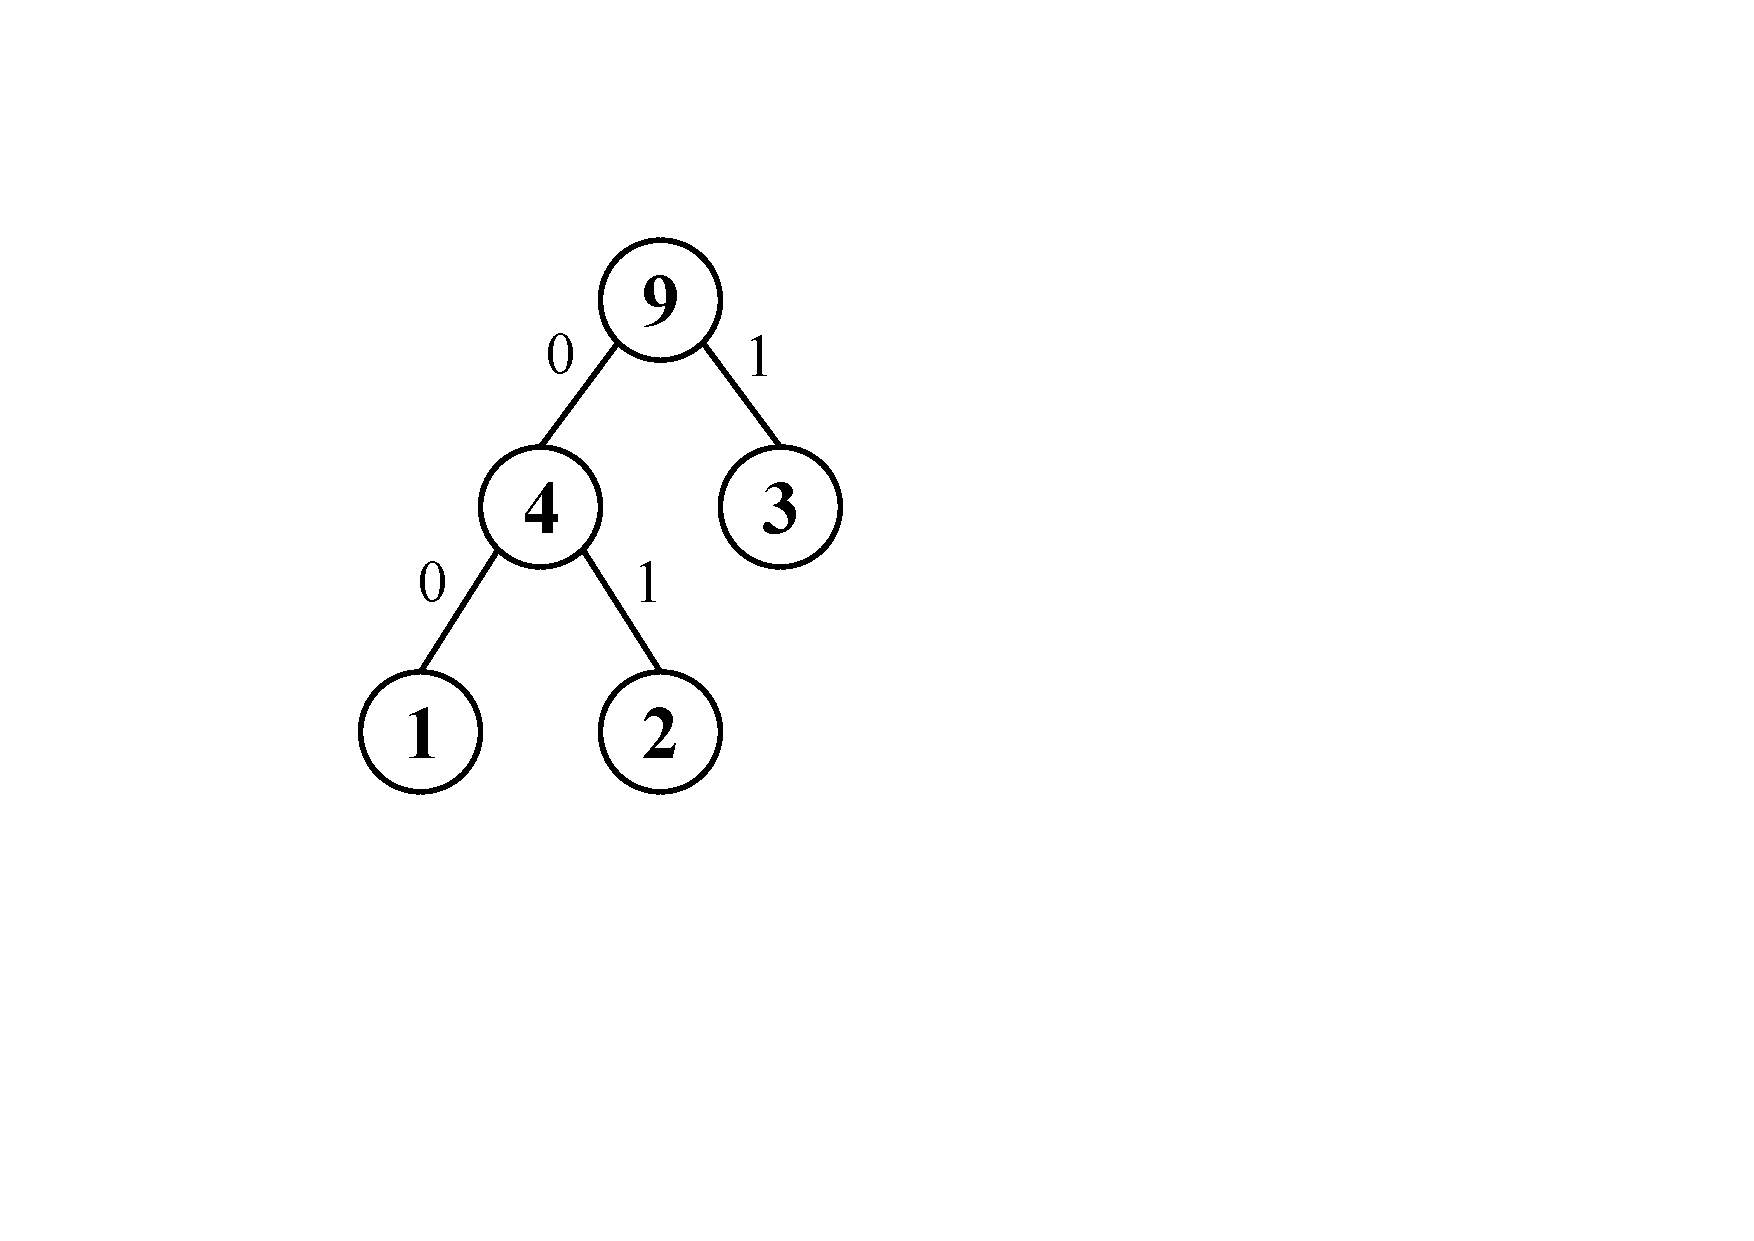
\includegraphics[scale=.4, clip, trim=160 200 410 100]{img/graphs-huffman.pdf}
    		
    		(c)
    	\end{minipage}

    \caption{Ejemplo de codificación Huffman. (a) Secuencia de entrada. (b) Secuencia de salida. (c) Diagrama de vocabulario en árbol binario.}
    \label{fig:huffman}
\end{figure}

